\documentclass[a4paper,11pt]{article}
\usepackage[margin=2cm]{geometry}
%\usepackage{anysize}
\usepackage[pdftex]{graphicx}
\usepackage{url}
\usepackage{fixltx2e}
\usepackage{listings}
\usepackage{textcomp}
\usepackage{wrapfig}
\usepackage{color}
\usepackage{subfig}
\usepackage{fancyhdr}
\usepackage{newclude}
\usepackage[nodayofweek]{datetime}
\usepackage[small,compact]{titlesec}
\usepackage[pdfborder=0]{hyperref}
\longdate

\setlength{\parskip}{11pt} 
\setlength\parindent{0pt}

\pagestyle{fancyplain}
\fancyhf{}
\lhead{\fancyplain{}{Machine Learning CBC}}
\rhead{\fancyplain{}{\today}}
\cfoot{\fancyplain{}{\thepage}}


\title{395 Machine Learning\\\Large{--- Assignment 4 ---}}
\author{Group 7\\Porfyrios Vasileiou, Afxentios Hadjiminas, John Flanagan.\\
       \{pv311, ah2411, jf311.\}@doc.ic.ac.uk\\ \\
       \small{CBC helper: Ioannis Marras}\\
       \small{Course: CO395, Imperial College London}
}


\begin{document}
\maketitle

\section{CBR Case Implementation}
For this assignment the case based reasoning (CBR) system is implemented as a
structure that contains an array of cases. Each case is a structure and holds
the problem vector which represents all the attributes that are set to 1. For
instance, if an example has positives only for the attributes 4, 10 and 18 then
the problem vector is stored as [4,10,28]. Furthermore, inside the case we also
store the full problem vector containing all the positive but negative
attributes as well. This enables us to apply the similarity measure functions
with more accuracy and flexibility. Lastly, inside the case structure there is
also the solution which is the actual label of the example, and the typicality
measure that helps us to choose amongst the cases with the same similarity.

\begin{center}
    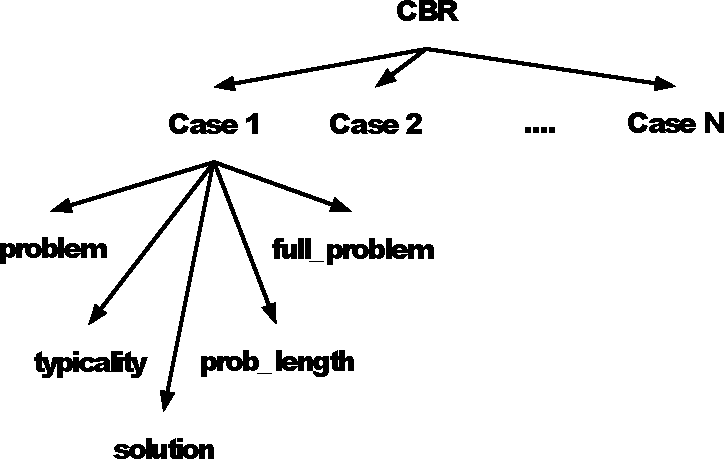
\includegraphics[width=.5\textwidth]{structure.pdf}
\end{center}
\section{CBR System Implementation}

\subsection{Retrieve Function}
The retrieve function takes as input the new case that has been converted from
an example and searches through the CBR to find the most similar case. This is
done using a similarity measure that compares the problem vectors of each case
in the CBR with the one given. The case that has the highest similarity is
returned. On many occasions there are cases with the same similarity measure
retrieved. When that happens, the ‘typicality measure’ is taken into account
and amongst those cases, the one with the higher typicality is returned.
Moreover, there are times when cases even have the same typicality and a new
measure has to be considered. This measure is the difference between the
problems of each candidate case with the one to classified. The case whose
problem length is closer to the tested case is returned.

\subsection{Reuse  Function}
The reuse function takes as input the most similar case returned by the
retrieve function as well as the case that is being classified. The solution
from the best case is then copied to the solution field of the new case which
is also the output of this function.

\subsection{Retain  Function}
After the case has been classified and therefore is solved we search through
the CBR system to check if it already exists as a unique case. This is done
using the created function findcase(cbr, case). If the cases exists, it is not
stored in the current CBR system but its typicality field is increased by one.
If it does not exist, the last index is found of the current CBR system and the
full solved case is stored in the last position(problem, full\_problem,
solution).

\section{Similarity Measures}

\subsection{Euclidean}
The first similarity measure that has been implemented and tested is the
euclidean distance otherwise known as the L2-norm. The distance between two
cases is calculated via the Pythagorean theorem which is the shortest distance
between two points. In this case, the difference between each couple of indices
is calculated and raised to the power of 2. In the end, the sum is computed and
the similarity measure is returned as the square root of the sum. The error
percentages of using the euclidean distance for the similarity measure, is
about 5\%-7\% which is very good. 

\begin{equation}
Euclidean Distance = \sqrt{\sum_i (c1(i) - c2(i))^{2})}
\end{equation}

\subsection{Manhattan}
Another similarity measure that has been tested is the city-block otherwise
known as the Manhattan distance(L1-norm). This measure sums the absolute
differences between each column of the full problems of the cases in
comparison. The one that has the smaller difference in total is considered to
be the most matching case. This method produces around the same error as the
one above at about 6\%.

\begin{equation}
Manhattan Distance = \sum_i |c1(i) - c2(i)|
\end{equation}

\subsection{Chebyshev}
The next similarity measure that has been implemented is the Chebyshev distance
(L-infinity-norm). This method iterates through each column of the cases that
are compared and finds the max absolute difference. Having the one with the
minimum maximum difference being returned. This measure produces an error of
about 80\%.

\begin{equation}
Chebyshev Distance = max_i |c1(i) - c2(i)|
\end{equation}

There are other similarity measures that can be implemented such as the problem
vector length but the above ones are the most important. From the results, the
Manhattan and Euclidean Distances have the same results with an error of about
6\%. On the other hand, the Chebyshev Distance does not work that well for this
specific problem. The reason that Manhattan and Euclidean distances have the
same error is because they rely on the same concept for calculating the
similarity. These methods appear to work really well because they compare each
column of the full problem, or each point, and use it to compute the minimum
distance between the two vectors. On the other hand, the Chebyshev measure
produces a big error due to the fact that for each case it finds the maximum
distance. This is not really effective.

\section{Overall Results}

\subsection{Precision and Recall Per Fold}
\begin{center}
\begin{tabular}{| l | c | c | c | c | c | c |} \hline
    & Anger & Disgust & Fear & Happiness & Sadness & Surprise \\ \hline
    Fold 1 &&&&&& \\ \hline
    Precision & 0.6667 & 0.7500 & 1.0000 & 1.0000 & 1.0000 & 1.0000 \\ \hline
    Recall & 0.6667 & 1.0000 & 0.5000 & 1.0000 & 1.0000 & 1.0000 \\ \hline
    &&&&&& \\ \hline
    Fold 2 &&&&&& \\ \hline
    Precision & 1.0000 & 1.0000 & 1.0000 & 1.0000 & 1.0000 & 1.0000 \\ \hline
    Recall & 1.0000 & 1.0000 & 1.0000 & 1.0000 & 1.0000 & 1.0000 \\ \hline
    &&&&&& \\ \hline
    Fold 3 &&&&&& \\ \hline
    Precision & 1.0000 & 1.0000 & 0.0000 & 1.0000 & 1.0000 & 1.0000 \\ \hline
    Recall & 0.5000 & 1.0000 & 1.0000 & 1.0000 & 1.0000 & 1.0000 \\ \hline
    &&&&&& \\ \hline
    Fold 4 &&&&&& \\ \hline
    Precision & 0.5000 & 1.0000 & 1.0000 & 1.0000 & 1.0000 & 1.0000 \\ \hline
    Recall & 0.5000 & 1.0000 & 0.0000 & 1.0000 & 1.0000 & 1.0000 \\ \hline
    &&&&&& \\ \hline
    Fold 5 &&&&&& \\ \hline
    Precision & 0.0000 & 1.0000 & 1.0000 & 1.0000 & 1.0000 & 1.0000 \\ \hline
    Recall & 0.5000 & 0.6667 & 1.0000 & 1.0000 & 1.0000 & 1.0000 \\ \hline
    &&&&&& \\ \hline
    Fold 6 &&&&&& \\ \hline
    Precision & 1.0000 & 1.0000 & 1.0000 & 1.0000 & 1.0000 & 1.0000 \\ \hline
    Recall & 1.0000 & 1.0000 & 1.0000 & 1.0000 & 1.0000 & 1.0000 \\ \hline
    &&&&&& \\ \hline
    Fold 7 &&&&&& \\ \hline
    Precision & 1.0000 & 1.0000 & 1.0000 & 1.0000 & 1.0000 & 1.0000 \\ \hline
    Recall & 1.0000 & 1.0000 & 1.0000 & 1.0000 & 1.0000 & 1.0000 \\ \hline
    &&&&&& \\ \hline
    Fold 8 &&&&&& \\ \hline
    Precision & 1.0000 & 1.0000 & 0.0000 & 1.0000 & 1.0000 & 1.0000 \\ \hline
    Recall & 1.0000 & 0.7500 & 1.0000 & 1.0000 & 1.0000 & 1.0000 \\ \hline
    &&&&&& \\ \hline
    Fold 9 &&&&&& \\ \hline
    Precision & 1.0000 & 1.0000 & 1.0000 & 1.0000 & 1.0000 & 1.0000 \\ \hline
    Recall & 1.0000 & 1.0000 & 1.0000 & 1.0000 & 1.0000 & 1.0000 \\ \hline
    &&&&&& \\ \hline
    Fold 10 &&&&&& \\ \hline
    Precision & 1.0000 & 1.0000 & 1.0000 & 1.0000 & 1.0000 & 1.0000 \\ \hline
    Recall & 1.0000 & 1.0000 & 1.0000 & 1.0000 & 1.0000 & 1.0000 \\ \hline
\end{tabular}
\end{center}
\subsection{Performance(F1Measure) Per Fold}

\begin{center}
    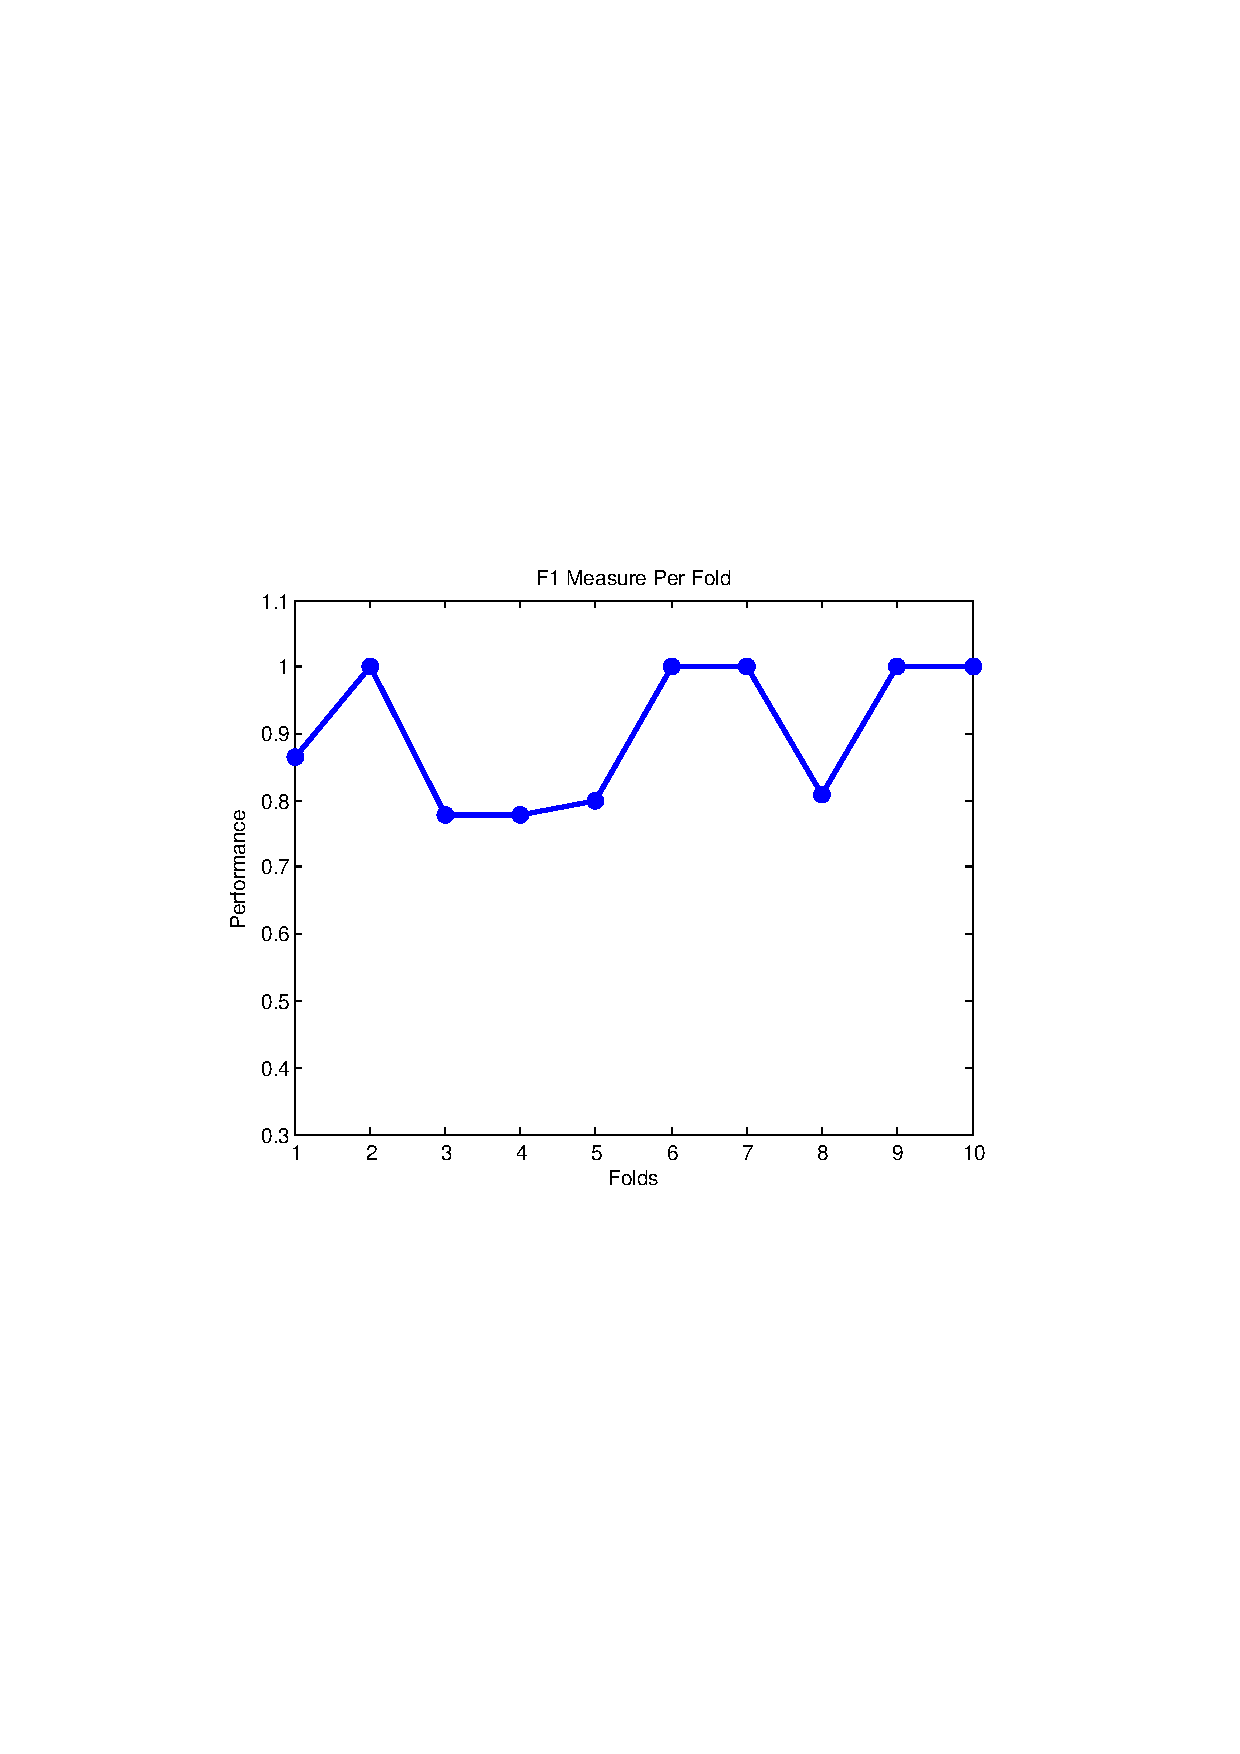
\includegraphics[width=.5\textwidth]{measure_per_fold.pdf}
\end{center}

\subsection{Average Confusion Matrix}
\begin{center}                                                                  
      \begin{tabular}{ | l || c | c | c | c | c | c | }                           
      \hline                                                                      
            & Anger 1 & Disgust 2 & Fear 3 & Happiness 4 & Sadness 5 & Surprise 6 \\ \hline \hline
          Anger 1 		& 10 & 1 & 1 & 0 & 0 & 0 \\ \hline                               
          Disgust 2 	& 1 & 20 & 1 & 0 & 0 & 0 \\ \hline                            
          Fear 3 		& 2 & 0 & 5 & 0 & 0 & 0 \\ \hline                                
          Happiness 4 	& 0 & 0 & 0 & 24 & 0 & 0 \\ \hline                          
          Sadness 5 	& 0 & 0 & 0 & 0 & 12 & 0 \\ \hline                             
          Surprise 6 	& 0 & 0 & 0 & 0 & 0 & 23 \\ \hline                           
     \end{tabular}                                                               
    \\ Average error: 0.06
\end{center}                                                                    

\subsection{Average Precision Recall F1Measure}

  \begin{center}                                                                  
  \begin{tabular}{ | l || c | c | c | c | c | c | }                               
     \hline                                                                      
        & Anger 1 & Disgust 2 & Fear 3 & Happiness 4 & Sadness 5 & Surprise 6 \\ \hline \hline
         Avg Recall                 & 0.7692 & 0.9524 & 0.7143 & 1.0000 & 1.0000 & 1.0000 \\ \hline   
         Avg Precision 				& 0.8333 & 0.9091 & 0.7143 & 1.0000 & 1.0000 & 1.0000 \\ \hline
        F\textsubscript{1} Measure  & 0.8000 & 0.9302 & 0.7143 & 1.0000 & 1.0000 & 1.0000 \\ \hline
      \end{tabular}                                                               
 \end{center}                                                                    


\end{document}
